\documentclass{beamer}
\usepackage{relsize}
\usepackage{color}

\usepackage{listings}
\usetheme{CambridgeUS}
%\usepackage{beamerthemesplit} % new
\usepackage{enumitem}
\usepackage{amsmath}                    % See geometry.pdf to learn the layout options.
\usepackage{amsthm}                   % See geometry.pdf to learn the layout options. There
\usepackage{amssymb}                    % See geometry.pdf to learn the layout options.
\usepackage[utf8]{inputenc}
\usepackage{graphicx}
\usepackage[english,bulgarian]{babel}

\lstset{language=C++,
                basicstyle=\ttfamily,
                keywordstyle=\color{blue}\ttfamily,
                stringstyle=\color{black}\ttfamily,
                commentstyle=\color{blue}\ttfamily,
                morecomment=[l][\color{magenta}]{\#}
}

\newtheorem{mydef}{Дефиниция}[section]
\newtheorem{lem}{Лема}[section]
\newtheorem{thm}{Твърдение}[section]

\DeclareMathOperator{\restrict}{\upharpoonright}

\setitemize{label=\usebeamerfont*{itemize item}%
  \usebeamercolor[fg]{itemize item}
  \usebeamertemplate{itemize item}}

\setbeamercovered{transparent}



\begin{document}
\title[Обектно ориентирано програмиране]{Представяне на функции и операции с тях}
\author{Калин Георгиев}
\frame{\titlepage}

\section{Абстракция за функция}

\begin{frame}
\centerline{Какво е функция?}
\end{frame}




\begin{frame}[fragile]
\frametitle{Изображение $f:A\rightarrow B$}

%\vspace{-60px}
\begin{center}
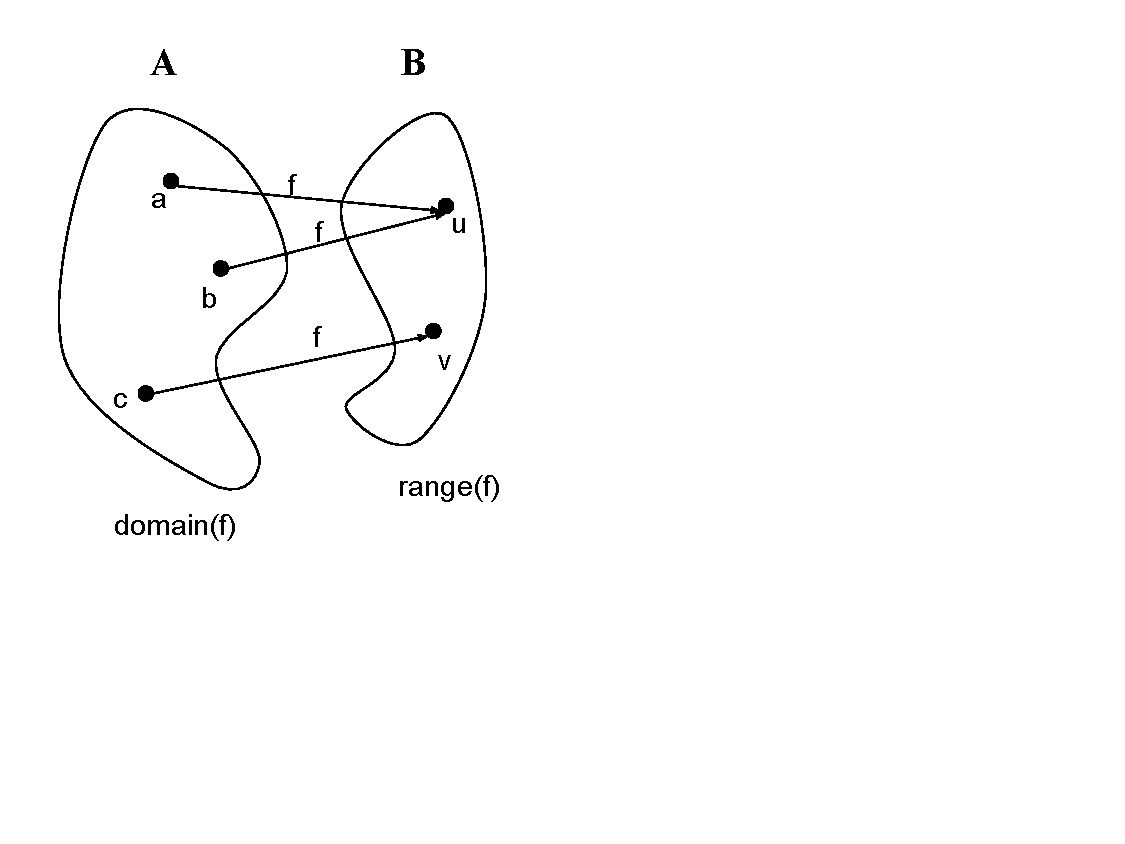
\includegraphics[width=12.0cm]{images/function_math}
\end{center}


\end{frame}



\begin{frame}[fragile]
\frametitle{Графика на функцията, $G(f)=\{(x,f(x))|x \in range(f)\}$}


\begin{columns}[t]
  \begin{column}{0.4\textwidth}
    \begin{center}
    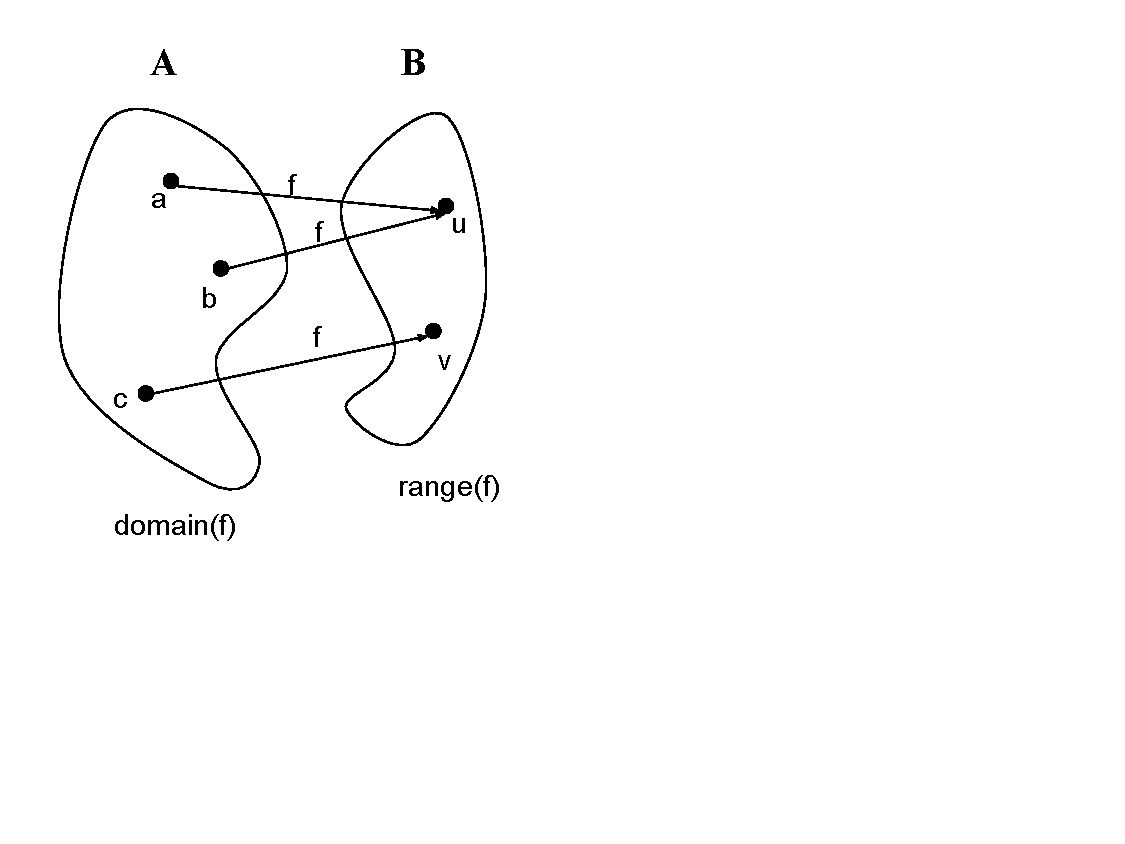
\includegraphics[width=9.0cm]{images/function_math}
    \end{center}
  \end{column}
  \begin{column}{0.6\textwidth}
    \begin{center}
    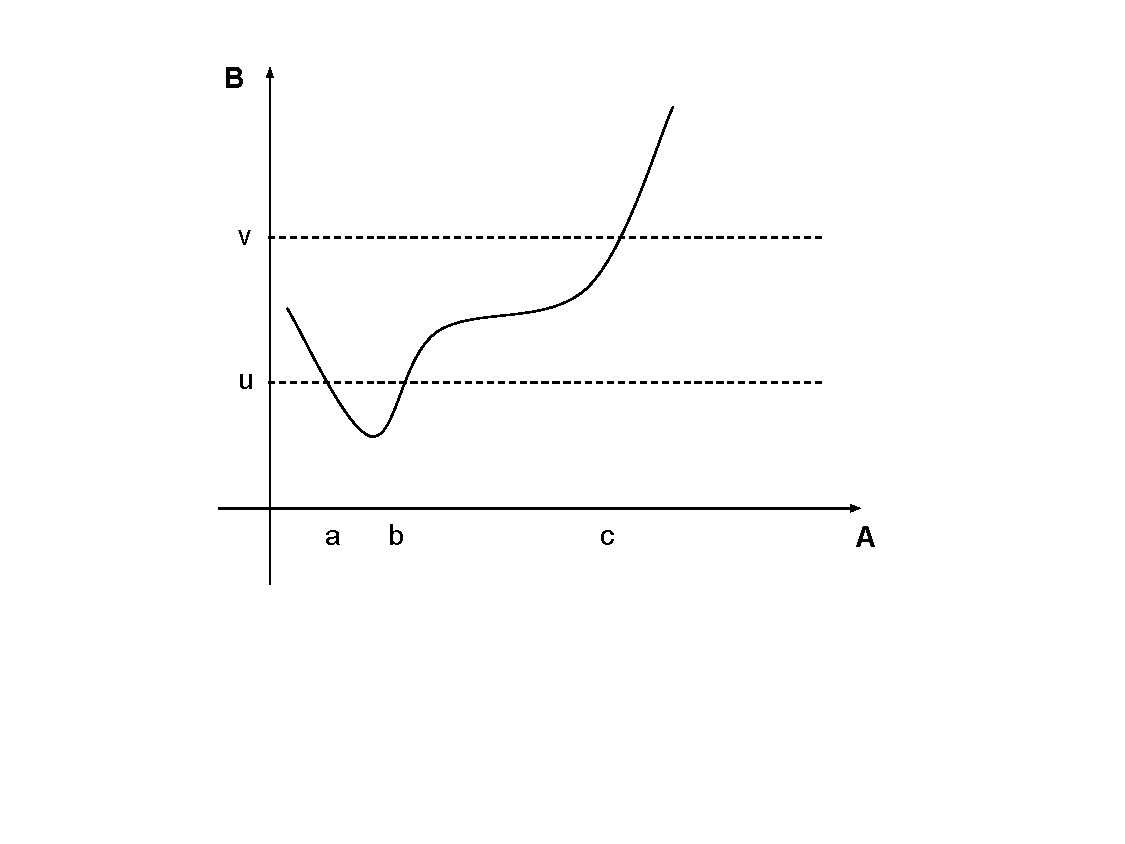
\includegraphics[width=9.0cm]{images/function_graph}
    \end{center}

  \end{column}
\end{columns}

%\vspace{-60px}

\end{frame}

\begin{frame}
\centerline{Как представяме функция компютърно?}
\end{frame}

\begin{frame}[fragile]
\frametitle{Таблично представяне}

\begin{center}
\begin{tabular}{c | c}
x & f(x) \\\hline
a & u \\
b & u \\
c & v
\end{tabular}

\end{center}


\end{frame}


\begin{frame}[fragile]
\frametitle{Представяне чрез програма}

\begin{center}
\begin{lstlisting}
double f (double x)
{
  if (x == a) return u;
  if (x == b) return u;
  if (x == c) return v;
  return 0;
}
\end{lstlisting}

\end{center}


\end{frame}


\begin{frame}
\centerline{Представяне на функцията чрез ``атрибути'',}
\centerline{които я дефинират еднозначно}
\end{frame}


\begin{frame}[fragile]
\frametitle{Константна функция}

\begin{center}

$f(x) = 5$

\begin{lstlisting}
class Constant
{
  private:
    double c;
  public:
    Constant (double val):c(val){}
}
\end{lstlisting}

\end{center}


\end{frame}


\begin{frame}[fragile]
\frametitle{Линейна функция}

\begin{center}

$f(x) = 2x + 5$

\begin{lstlisting}
class Linear
{
  private:
    double coef;
    double constant;
  public:
    Linear (double a,double b):
       coef(a),constant(b){}
}
\end{lstlisting}

\end{center}


\end{frame}



\begin{frame}[fragile]
\frametitle{Полином}

\begin{center}

$f(x) = a_0x^n + a_1x^{n-1}+...+a_n$

\begin{lstlisting}
class Polynom
{
  private:
    vector<double> coefs;
  public:
    Polynom (vector<double>arr):
       coefs(arr){}
}
\end{lstlisting}

\end{center}


\end{frame}


\begin{frame}
\centerline{Кое е общото между всички}
\centerline{едноместни числови функции?}
\end{frame}



\begin{frame}[fragile]
\frametitle{$y=f(x)$}

\begin{center}

\begin{lstlisting}
class Function
{
  public:
  virtual double value (double x) = 0;
}
\end{lstlisting}

\end{center}


\end{frame}



\begin{frame}[fragile]
\frametitle{Константна функция}

\begin{center}

$f(x) = 5$

\begin{lstlisting}
class Constant : public Funtion
{
  private:
    double c;
  public:
    Constant (double val):c(val){}

    double value (double x) {return c};
}
\end{lstlisting}

\end{center}


\end{frame}


\begin{frame}[fragile]
\frametitle{Линейна функция}

\begin{center}

$f(x) = 2x + 5$

\begin{lstlisting}
class Linear : public Funtion
{
  private:
    double coef;
    double constant;
  public:
    Linear (double a,double b):
       coef(a),constant(b){}

    double value (double x)
    {
      retuen coef*x + constant;
    }
}
\end{lstlisting}

\end{center}


\end{frame}



\begin{frame}[fragile]
\frametitle{Полином}

\begin{center}

$f(x) = a_0x^n + a_1x^{n-1}+...+a_n$

\begin{lstlisting}
class Polynom : public Funtion
{/...
    double value (double x)
    {
      double sum = coefs[0];
      for (int i = 1; i < coefs.size()-1; i++)
        sum = sum * x + coefs[i];
      return sum;
    }
}
\end{lstlisting}

\end{center}


\end{frame}




\begin{frame}
\centerline{Оператори над функции}
\end{frame}


\begin{frame}[fragile]
\frametitle{Функция vs. Оператор}

\begin{itemize}
  \item Функция: $f:A\rightarrow B$, $g:B\rightarrow C$
  \item Оператор: $\Gamma:(A\rightarrow B)\rightarrow (A\rightarrow B)$
  \item Оператор: $\Gamma:(A\rightarrow B)\times(B\rightarrow C)\rightarrow (A\rightarrow C)$
\end{itemize}

\end{frame}



\begin{frame}[fragile]
\frametitle{$\Gamma:(double \rightarrow double)\rightarrow(double \rightarrow double)$}

\begin{center}
$$
\Gamma(f)(x) = \left\{
        \begin{array}{ll}
            f(x) & \quad f(x) \geq 0 \\
            0 & \quad otherwise
        \end{array}
    \right.
$$

\relscale{0.95}
\begin{lstlisting}
class CutFunction : public Function
{
  private:
    Function* f;
  public:
    CutFunction (Function *_f):f(_f){}
    double value (double x){
      double y = f->value(x);
      if (y >= 0)
        return y;
      return 0;
    }
}
\end{lstlisting}

\end{center}


\end{frame}


\begin{frame}[fragile]
\frametitle{Използване на CutFunction}


\begin{columns}[t]
  \begin{column}{0.50\textwidth}


      \begin{flushleft}
      \relscale{0.85}
\begin{lstlisting}
class CutFunction : public Function
{
  private:
    Function* f;
  public:
    CutFunction (Function *_f):f(_f){}
    double value (double x){
      double y = f->value(x);
      if (y >= 0)
        return y;
      return 0;
    }
}
\end{lstlisting}

      \end{flushleft}

  \end{column}
  \begin{column}{0.5\textwidth}
      \begin{flushleft}

      \relscale{0.80}
      \begin{lstlisting}
      int main ()
      {
        Linear fn (-2,10);
        CutFunction cfn (&fn);

        cout << fn.value (10)
             << endl
             << cfn.value (10);
      }
      \end{lstlisting}

      \end{flushleft}

  \end{column}
\end{columns}



\end{frame}

\begin{frame}[fragile]
\frametitle{$f$ и $CutFn(f)$ са фунцкии}


\begin{flushleft}
\relscale{1}
\begin{lstlisting}
void printall (Function *functions[],
               int n,
               double x)
{
  for (int i = 0; i < n; i++)
    cout << functions[i]->value(x) << endl;
}
int main ()
{
  Linear fn (-2,10);
  CutFunction cfn (&fn);
  Function *functions[] = {&fn,&cfn};
  printall (functions,2,10);
}
\end{lstlisting}

\end{flushleft}
\end{frame}







\begin{frame}[fragile]
\frametitle{$\Gamma:(double \rightarrow double) \times (double \rightarrow double) \rightarrow(double \rightarrow double)$}

\begin{center}
$$
\Gamma(f,g)(x) = f(g(x))
$$

\relscale{0.95}
\begin{lstlisting}
class Composition : public Function
{
  private:
    Function* f;
    Function* g;
  public:
    Composition (Function *_f, Function *_g)
        :f(_f),g(_g){}
    double value (double x){
      return f->value (g->value (x));
    }
}
\end{lstlisting}

\end{center}


\end{frame}


\begin{frame}[fragile]
\frametitle{Използване на Composition}


\begin{flushleft}

\relscale{0.80}
\begin{lstlisting}
int main ()
{
  Linear fn (-2,10);
  CutFunction cfn (&fn);
  Composition comp (&fn,&cfn);

  cout << comp.value (10);

  Function *functions[] = {&fn,&cfn,&comp};
  printall (functions,3,10);

}
\end{lstlisting}

\end{flushleft}


\end{frame}












\begin{frame}
\centerline{Програмите като оператори}
\end{frame}


\begin{frame}[fragile]
\frametitle{IF като oператор}

\begin{center}

\relscale{0.95}
\begin{lstlisting}
double G (double x)
{
  if (f(x) != 0)
    return g(x);
  return h(x);
}
\end{lstlisting}

\end{center}


$$
\Gamma(f,g,h)(x) = \left\{
        \begin{array}{ll}
            g(x) & \quad f(x) \neq 0 \\
            h(x) & \quad otherwise
        \end{array}
    \right.
$$



\end{frame}




\begin{frame}[fragile]
\frametitle{IF като оператор}

\begin{center}
$$
\Gamma(f,g,h)(x) = \left\{
        \begin{array}{ll}
            g(x) & \quad f(x) \neq 0 \\
            h(x) & \quad otherwise
        \end{array}
    \right.
$$


\relscale{0.95}
\begin{lstlisting}
class IfOperator : public Function
{
  private:
    Function* condfn; //f
    Function* thenfn; //g
    Function* elsefn; //h
  public:
    IfOperator (Function *_c,
                Function *_t,
                Function *_e):condfn(_c),
                              thenfn(_t),
                              elsefn(_e){}
}
\end{lstlisting}

\end{center}


\end{frame}





\begin{frame}[fragile]
\frametitle{IF като оператор}

\begin{center}
$$
\Gamma(f,g,h)(x) = \left\{
        \begin{array}{ll}
            g(x) & \quad f(x) \neq 0 \\
            h(x) & \quad otherwise
        \end{array}
    \right.
$$


\relscale{0.95}
\begin{lstlisting}
class IfOperator : public Function
{
  public:
    double value (double x){
      if (condfn->value(x) == 0)
        return elsefn->value (x);
      return thenfn->value (x);
    }
}
\end{lstlisting}

\end{center}


\end{frame}



\begin{frame}[fragile]
\frametitle{FOR като ператор}

\begin{center}

\relscale{0.95}
\begin{lstlisting}
double G (double x)
{
  double z = x;
  for (int i = 0; i < N; i++)
    z = f(z);
  return z;
}
\end{lstlisting}

\end{center}


$$
\Gamma(f,n)(x) = \underbrace{f(f...(f}_n(x)..)
$$



\end{frame}




\begin{frame}[fragile]
\frametitle{FOR като оператор}

\begin{center}

$$
\Gamma(f,n)(x) = \underbrace{f(f...(f}_n(x)..)
$$



\relscale{0.85}
\begin{lstlisting}
class ForOperator : public Function
{
  private:
    Function* fn;
    int count;
  public:
    ForOperator (Function *_fn):fn(_fn){}
    double value (double x)
    {
      double z  = x;
      for (int i = 0; i < count; i++)
        z = fn->value(z);
      return z;
    }
}
\end{lstlisting}

\end{center}


\end{frame}



%%   \begin{frame}[fragile]
%%   \frametitle{WHILE като ператор}
%%   
%%   \begin{center}
%%   
%%   \relscale{0.95}
%%   \begin{lstlisting}
%%   double G (double x)
%%   {
  %%   z = x;
  %%   while (h(z) != 0)
  %%   {
    %%   z = f(z);
  %%   }
  %%   return z;
%%   }
%%   \end{lstlisting}
%%   
%%   \end{center}
%%   
%%   
%%   $$
%%   \Gamma(f,h)(x) = \left\{
        %%   \begin{array}{ll}
            %%   x & \quad h(x) == 0 \\
            %%   \Gamma(f,h)(f(x)) & \quad otherwise
        %%   \end{array}
    %%   \right.
%%   $$
%%   
%%   
%%   
%%   \end{frame}
%%   
%%   
%%   \begin{frame}[fragile]
%%   \frametitle{WHILE като оператор}
%%   
%%   \begin{center}
%%   $$
%%   \Gamma(f,h)(x) = \left\{
        %%   \begin{array}{ll}
            %%   x & \quad h(x) == 0 \\
            %%   \Gamma(f,h)(f(x)) & \quad otherwise
        %%   \end{array}
    %%   \right.
%%   $$
%%   
%%   
%%   \relscale{0.95}
%%   \begin{lstlisting}
%%   class WhileOperator : public Function
%%   {
  %%   private:
    %%   Function* condfn;
    %%   Function* operation;
  %%   public:
    %%   WhileOperator (Function *_c,
                   %%   Function *_o):condfn(_c),
                                 %%   operation(_o){};
%%   }
%%   \end{lstlisting}
%%   
%%   \end{center}
%%   
%%   
%%   \end{frame}
%%   
%%   
%%   
%%   \begin{frame}[fragile]
%%   \frametitle{WHILE като оператор}
%%   
%%   \begin{center}
%%   
%%   $$
%%   \Gamma(f,h)(x) = \left\{
        %%   \begin{array}{ll}
            %%   x & \quad h(x) == 0 \\
            %%   \Gamma(f,h)(f(x)) & \quad otherwise
        %%   \end{array}
    %%   \right.
%%   $$
%%   
%%   
%%   \relscale{0.95}
%%   \begin{lstlisting}
%%   class WhileOperator : public Function
%%   {
    %%   double value (double x)
    %%   {
      %%   double z  = x;
      %%   while (condfn->value(z))
        %%   z = operation->value(z);
      %%   return z;
    %%   }
%%   }
%%   \end{lstlisting}
%%   
%%   \end{center}
%%   
%%   
%%   \end{frame}


\begin{frame}
\centerline{Благодаря ви за вниманието!}
\end{frame}

\end{document}



\begin{columns}[t]
  \begin{column}{0.55\textwidth}

  \end{column}
  \begin{column}{0.45\textwidth}

  \end{column}
\end{columns}
